\documentclass[12pt]{article}
\usepackage{amsmath}
\usepackage{graphicx}
\title{Report for Auto Control Lab8}
\date{2020/11/10}
\author{Jacky Yeh 4107064003}

\begin{document}
\begin{titlepage}

\maketitle
\end{titlepage}


\section{Introduction}
This is the tenth Experiment of Auto Control Lab where TAs taught us the plot some characteristics of the system which includes steady-state error and also and some optimal value of percent-overshoot.


\section{LAB7}
\subsection{Part 1 Homework problems and its codes}
Objective:To perform operations to find out the steady state error plot\\

These are the stated Homework problems\\

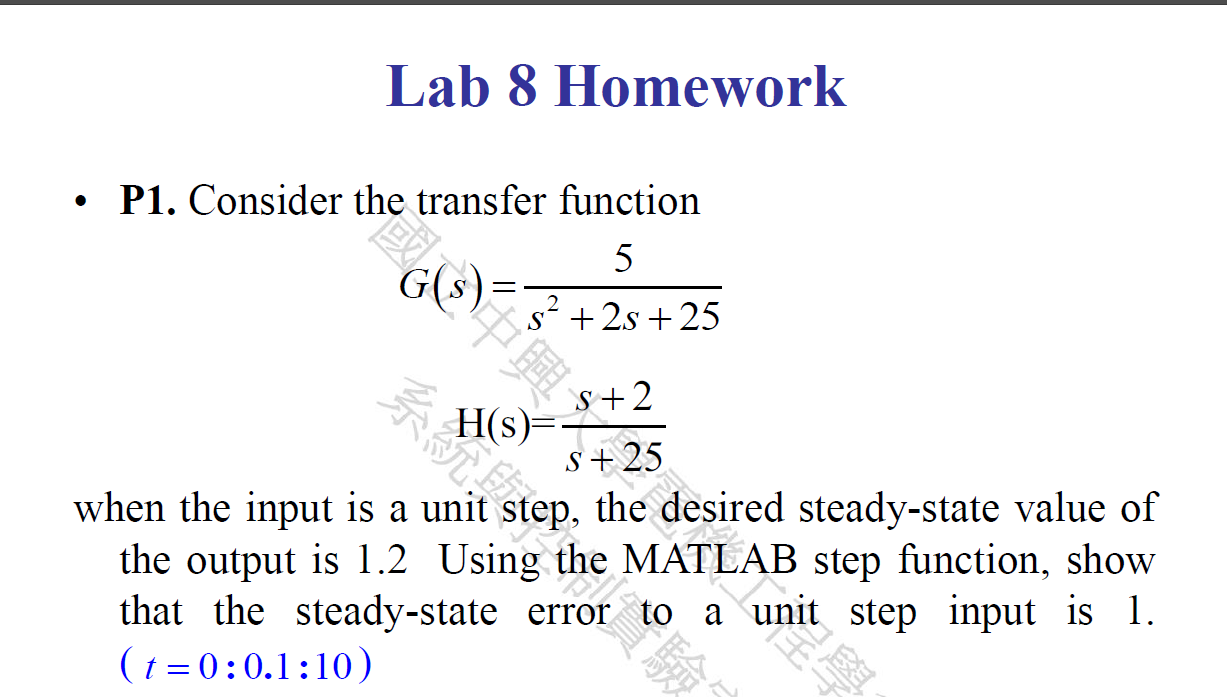
\includegraphics[scale=0.6]{../Lab8/Pictures/LabProblem1.png} \\

\cleardoublepage

\subsection{CODES FOR PROBLEM1}
In order to perform the tasks, Matlab codes are needed. The following is the code needed for finding the steady state error plot which I minus the desired output with my real output\\

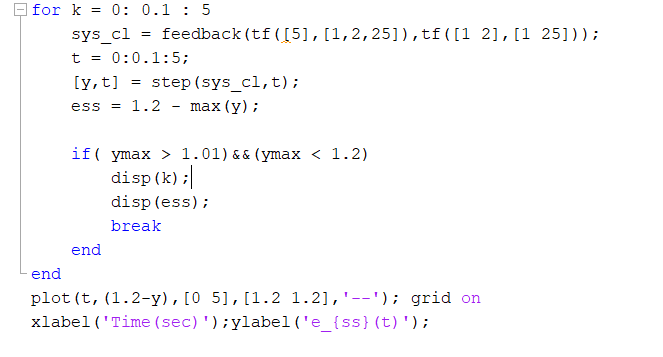
\includegraphics[scale=0.4]{../Lab8/Pictures/LabProblem1Code1.png} \\ 

\subsection{Result of the given difference of desired output and my real output i.e 1.2-y} 

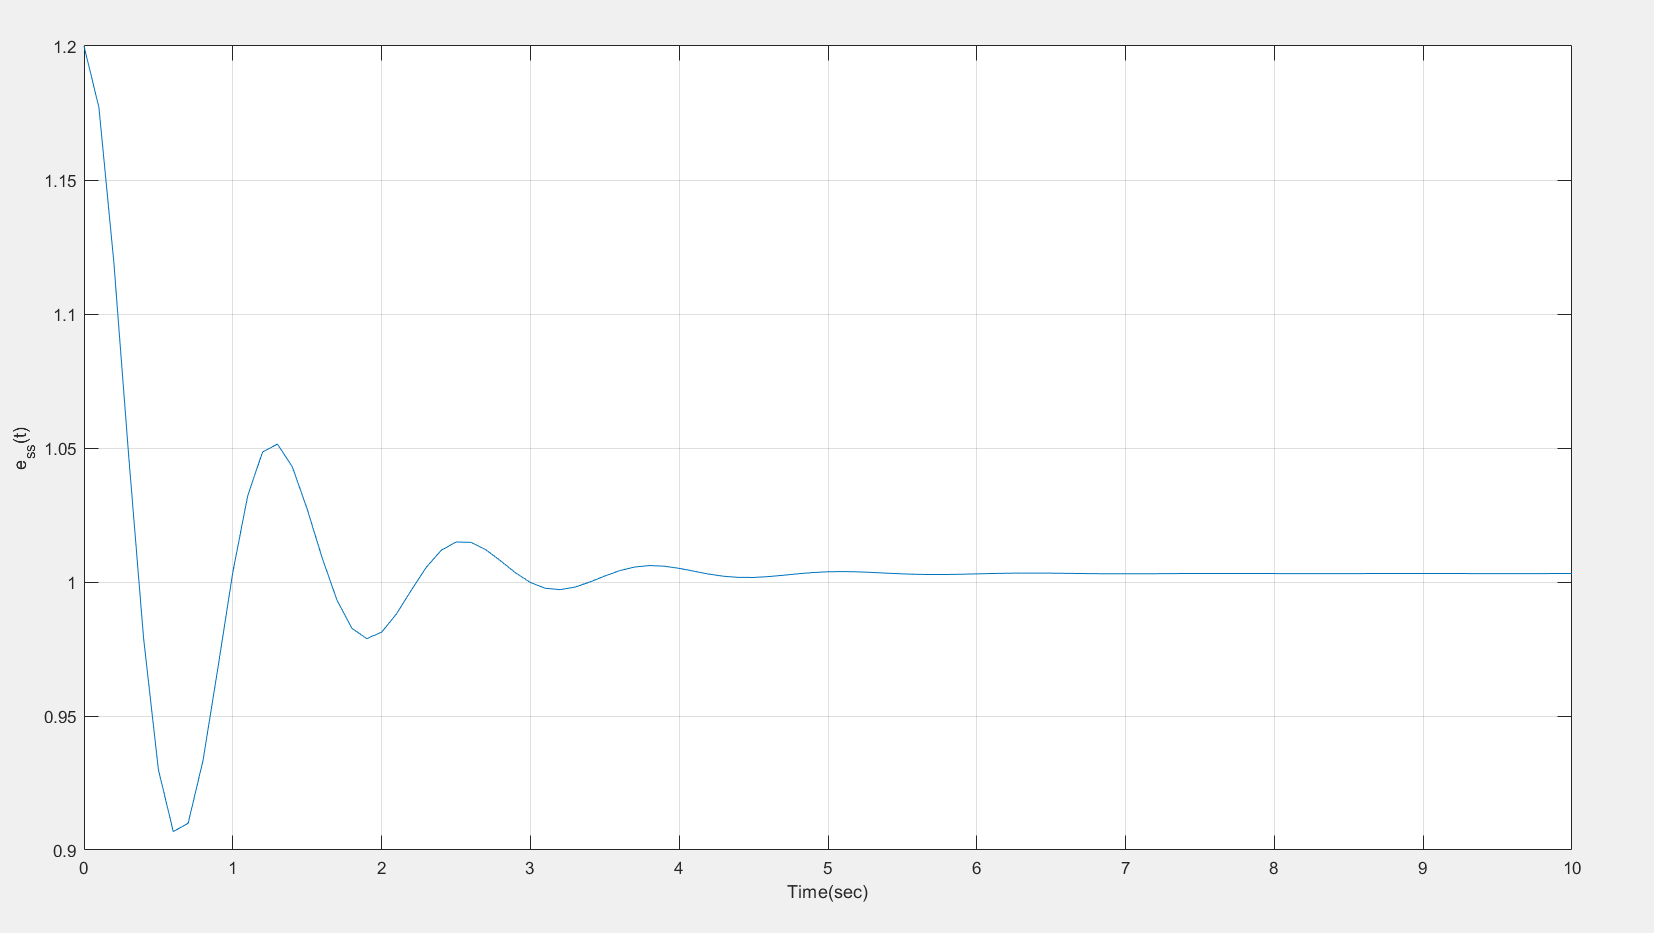
\includegraphics[scale=0.4]{../Lab8/Pictures/LabProblem1Result1.png}  \\ 


\cleardoublepage



 
\cleardoublepage
\subsection{Part 2 Homework problems and its codes}
Objective:To plug in and plot out the response with the given feedback system to a step response and find the optimal value of k to be in the percent overshoot range ,also have to plot out the steady state error for the last value of k\\
These are the stated HW problems.

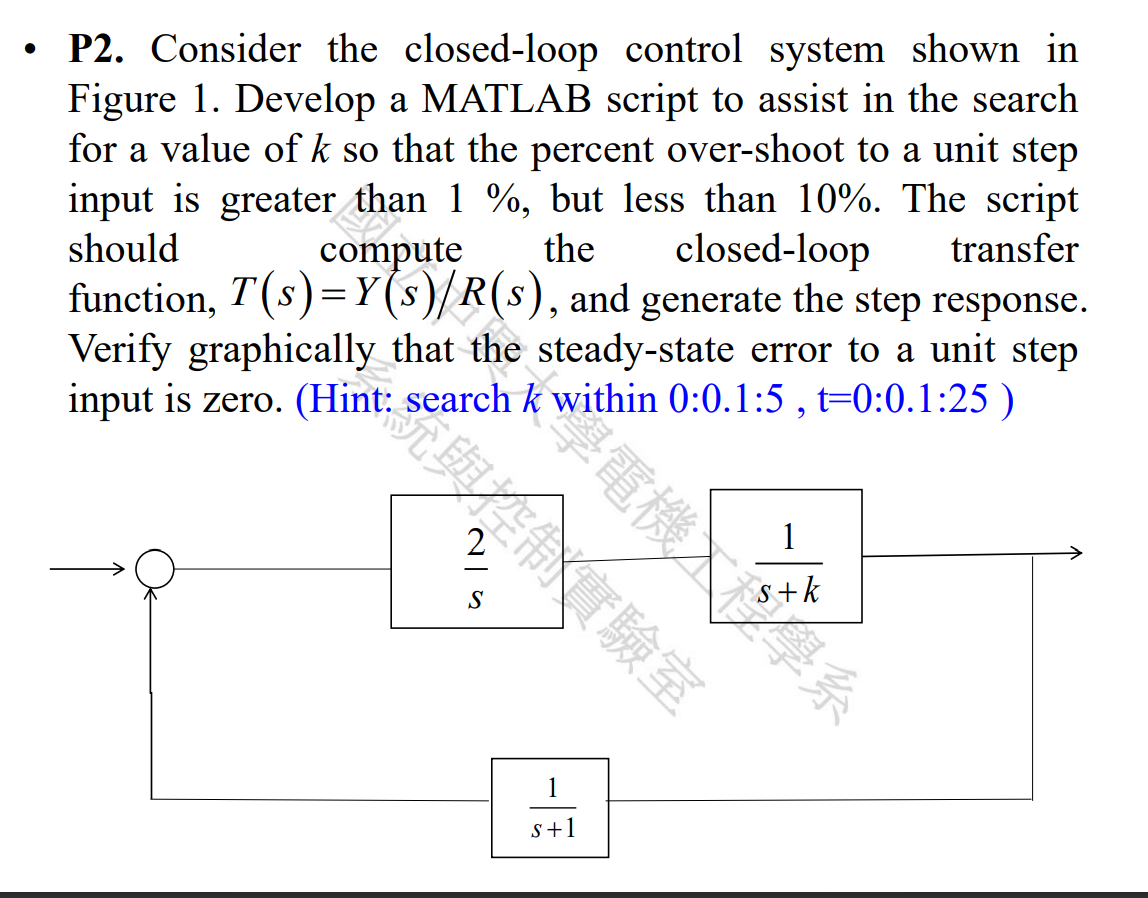
\includegraphics[scale=0.5]{../Lab8/Pictures/LabProblem2.png} \\


\cleardoublepage
\subsection{CODES FOR Part2}
In order to perform the tasks, Matlab codes are needed. The following code is used for finding the value k and also to plot the system out with step response also the steady state error \\

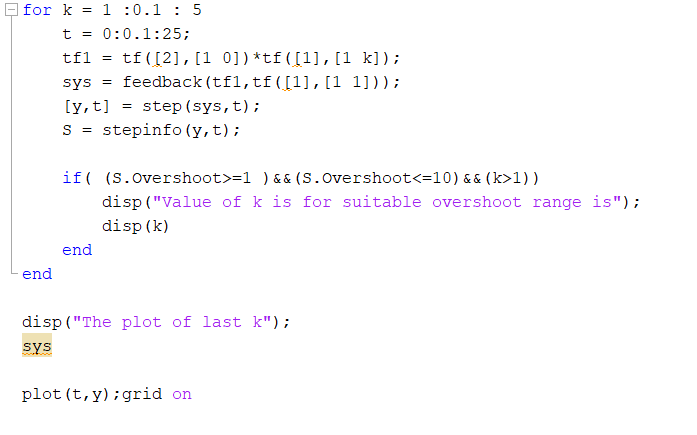
\includegraphics[scale=0.5]{../Lab8/Pictures/LabProblem2Code.png} 


\subsection{Plot Response OF the given system and the state transition matrix PHI} 
Optimal value of k's\\

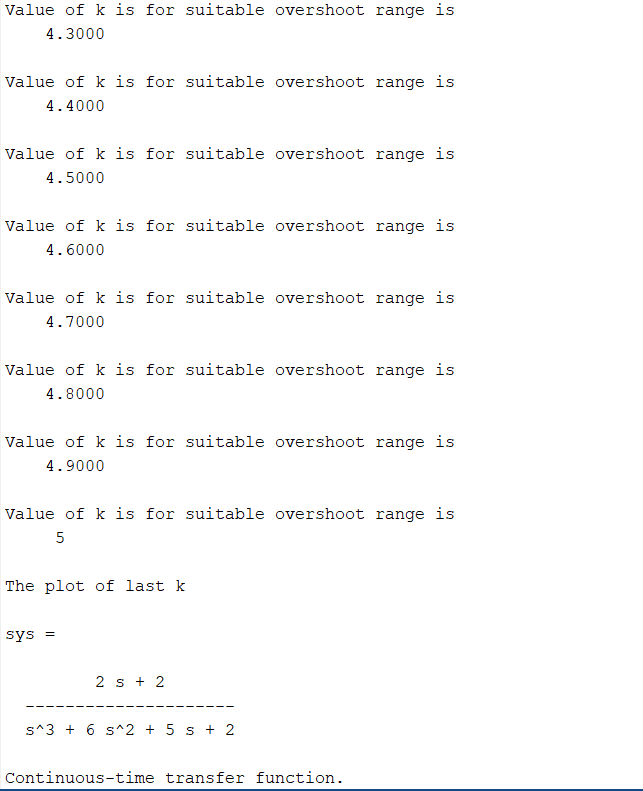
\includegraphics[scale=0.4]{../Lab8/Pictures/LabProblem2Result_Valueofk_and_sys.png}   \\

\cleardoublepage
The following is the system out given\\

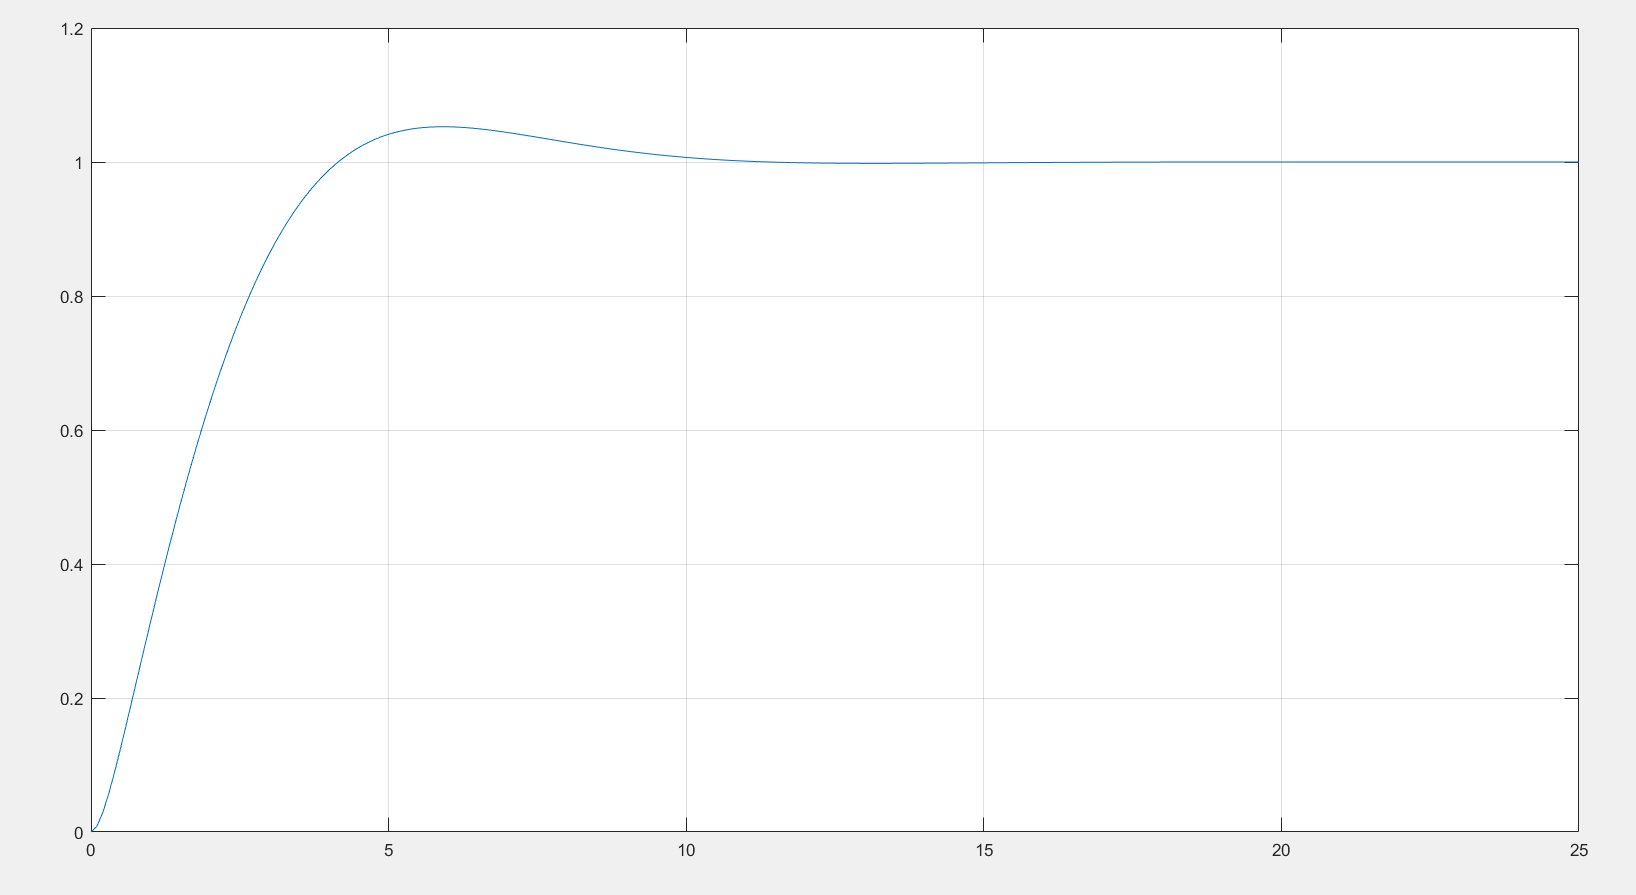
\includegraphics[scale=0.4]{../Lab8/Pictures/LabProblem2Result1_Transfer_Funtion_plot.png}  \\

The following is the system steady state error which approach to zero\\

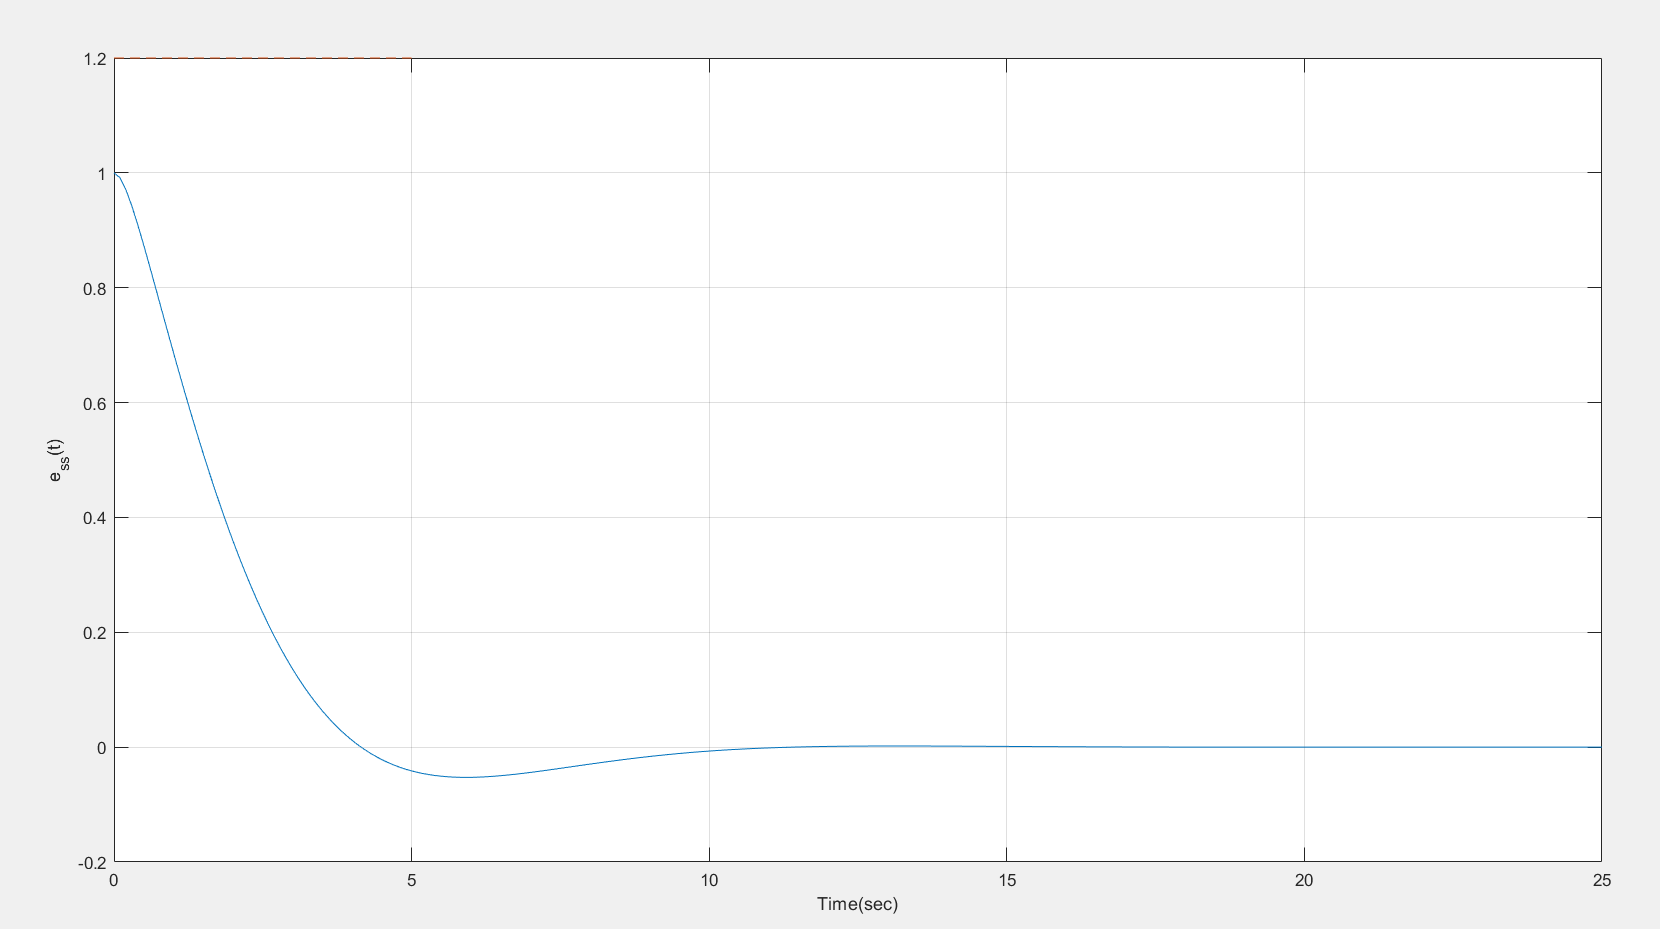
\includegraphics[scale=0.4]{../Lab8/Pictures/LabProblem2Result_steady_state_error.png} 


\section{Conclusion}
Today we learn how to find the characteristics of a certain system to some certain inputs. Which includes some important concept about percent overshoot and also steady state error plot. However, some materials shall also be included which are the peak time,settling time and rise time etc.... Anyways, with the help of the auto control course, it is easier for me to grasp those idea, and also help me cement the ideas of features of the system learnt in control system course.

\begin{center} 
This concludes the tenth Week of Auto Control LAB\\
\end{center}

\end{document} 
